
Der Begriff Lumineszenz leitet sich vom lateinischen \emph{lumen}= kaltes Licht ab und bezeichnet eine außergenwöhnliche Leuchterscheinung unterhalb der Glühtemperatur, die beim Übergang vom angeregten Zustand zum Grundzustand entsteht. Je nach Anregung  unterscheidet man verschiedene Arten von Lumineszenz.
\section{Arten der Lumineszenz}
\textbf{Photolumineszenz (Fluoreszenz,Phosphoreszenz):}
\\Lichtabsorption bewirkt, dass das Material elektronisch angeregt wird und dann durch spontane Photonen-Emission (Licht wird ausgesendet in niedrigere Energiezustände zurückkehrt. 
\\\textbf{Radiolumineszenz:}
\\Ein Stoff kann durch Ionisationsstrahlen angeregt werden. Dies läuft ähnlich wie bei der Thermolumineszenz ab.
\\\textbf{Kathodolumineszenz:}
\\Ein Elektronenstrahl kommt aus einer Elektronenquelle und prahlt auf eine
Festkörperoberfläche auf und worauf diese dazu angeregt wird, Licht auszusenden.
\\\textbf{Elektrolumineszenz:}
\\Sie ist auch unter dem Begriff Destriau-Effekt bekannt. Wird ein elektrisches Feld an einen Feskörper angelegt, wird dieser dazu verleitet elekromagnetische Strahlung auszusenden. Durch Wechsel- oder Gleichspannung kann diese Art der Anregung erfolgen.
\\\textbf{Thermolumineszenz:}
\\Nach Speicherung der Energie im Kristallgitter, kann diese durch Erhitzung freigesetzt werden.
\\\textbf{Chemilumineszenz:}
\\Durch einen chemischen Prozess wird sichtbares Licht emittiert. Ausgangsstoffe für Chemilumineszenz-Reaktionen sind Luminophore. Bei den meisten Chemilumineszenz-Reaktionen entsteht zunächst ein instabiles Intermediat mit einer Peroxid-Brücke, dessen energiereiches Zerfallsprodukt einen Charge-Transfer-Komplex mit einem Farbstoffmolekül bildet und Energie an dieses abgibt. Das angeregte Farbstoffmolekül sendet dann ein Lichtquant aus, dessen Wellenlänge von der Struktur des verwendeten Farbstoffs abhängt.
\\\textbf{Biolumineszenz:}
\\Sie ist eine Form der Chemilumineszenz und beschreibt die Fähigkeit von Lebewesen selbst oder mit Hilfe von Symbionten Licht zu erzeugen. Wenn das Tier zum Selbstleuchten in der Lage ist, bezeichnet man dies als primäres Leuchten. Wenn jedoch das Leuchten durch symbiontische Bakterien ensteht, wird es sekundäres Leuchten genannt. \cite{[1]}

\section{physikalisch-chemische Grundlagen}
Elektromagnetische Strahlung kann ein Molekül in einen elektronisch angeregten Zustand versetzen. Die Rückkehr des Systems in den Grundzustand kann durch spontane oder stimulierte Emission passieren.
Zwischen LUMO (lowest occupied molecule orbital) und HOMO (highest occupied molecule orbital) ist der Energieunterschied größer als die Anregungsenergie A für den Übergang vom Singulett-Grundzustand $S_0$ in den ersten elektronisch angeregten Singulettzustand $S_1$. Durch verschiedene Elektronen-Wechselwirkungen  wie der Coloumb-Term J oder Austauschterm 2K) kann dies ausgedrückt werden. Die Aufspaltung von Singulett und Triplett ergibt näherungsweise 2 K. Der unterste Triplettzustand ($T_1$) befindet sich immer unter dem ersten Singulett-Zustand ($S_1$), weil K größer als 0 ist. Die Anregungsenergien von Molekülen mit gleichem HOMO-LUMO-Abstand können unterschiedlich sein. Der Übergang zwischen HOMO und LUMO ist nicht gleich $S_0$ $\rightarrow$ $S_1$ (energieärmster Übergang),was an der Konfigurationswechselwirkung liegt.
\\Wie bei Atomen sind für zwei- oder linear mehratomige Moleküle Auswahlregeln aufgestellt worden,die erlaubten Übergänge zwischen zwei verschiedenen elektronischen Zuständen aufzeigen.
\\\textbf{1.Spinverbot:} Während des Übergangs ist die Veränderung von Gesamtspin S und Multiplizität ($M=2S+1$) nicht erlaubt. Singulettzustände dürfen in Singulettzustände, nicht aber in Triplettzustände übergehen.
\\\textbf{2.Symmetrie-Verbot:} Elektronenübergänge zwischen Orbitalen gleicher Parität sind verboten, z.B. sind g $\rightarrow$u, u$\rightarrow$g- Übergänge erlaubt, aber g$\rightarrow$g, u$\rightarrow$u-Übergänge nicht(g = symmetrisch, u = unsymmetrisch bezüglich ihrer Inversion). Die Erniedrigung der Symmetrie kann durch Kernbewegungen bewirkt werden und so können diese verbotenen Übergänge doch stattfinden.
\\\textbf{3.Üpperlappungsverbot}: Wenn sich die beiden Orbitale, die sich im Elektronenübergang befinden, nicht oder nur kaum räumlich überlappen, so tritt das Verbot ein. Beobachtbar ist dies bei intermolekularen Charge-Transfer-Übergangen, bei dem im Komplex der Elektronenübergang vom Donator- auf das Akzeptor-Molekül erfolgt.
\\Die verschiedene Übergänge von Elektronen zeigen, dass die Verbote die Regel und erlaubte Übergänge nur Ausnahmen sind. \cite{[2]}

\newpage
\section{Übergänge zwischen elektronischen Zuständen}
Findet Anregung bei einem Molekül statt, kann es zum Grundzustand zurückkehren oder über andere Wege aus dem angeregten Zustand austreten. Das Perrin-Jablonsky-Termschema kann diese Übergänge darstellen:

\begin{figure}[htbp]
\centering
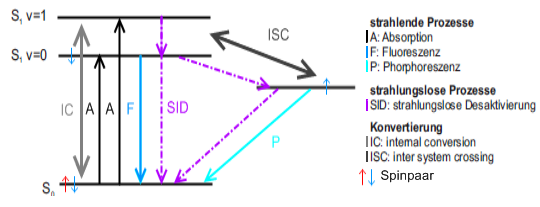
\includegraphics[scale=0.5]{graphics/Jablonski_Termschema}
\caption{Jablonsky-Termschema \cite{[3]} } 
\end{figure}

Die Singulett-Zustände werden dabei als $S_0$ (Grundzustand),$S_1, S_2$...und die Triplett-Zustände als $T_1, T_2$ bezeichnet. Auf einige dieser Vorgänge wird genauer eingegangen.
\subsection{internal conversion}
Dabei handelt es sich um einen Übergang ohne Strahlung zwischen zwei elektronischen Zuständen mit der gleichen Spinmultiplizität. Auf diesen Prozess folgt in Lösung eine Schwingungsrelaxation auf den niedrigsten Schwingungslevel des letzten elektronischen Zustandes. Stösst das angeregte Molekül mit Lösungsmittelmolekülen zusammen, kann die Schwingungsenergie übertragen werden. Wegen des großen Energieunterschiedes ist internal conversion vom $S_1$ in den Grundzustand zwar möglich, aber nicht sehr effektiv. Übergänge $S_2$ $\rightarrow$ $S_1$ findet daher eher statt. Interne Conversion von $S_1$ zu $S_0$ steht in direkter Konkurrenz zu Fluoreszenz und zu intersystem crossing.
\subsection{Fluoreszenz}
Als Fluoreszenz bezeichnet man das Aussenden von Photonen bei der Rückkehr von $S_1$- in den $S_0$-Zustand. Das Fluoreszenzspektrum liegt auf höheren Wellenlängen (niedrigerer Energie) als das Absorptionsspektrum, weil Energie durch Schwingungsrelaxation verlorengeht. In den meisten Fällen überlappt das Absorptionsspektrum teilweise das Fluoreszenzspektrum, was laut der Stokes-Regel nicht sein sollte. Der Abstand (ausgedrückt in Wellenzahlen) zwischen dem ersten Absorptionsband und dem Maximum des Fluoreszenzbandes wird als Stokesshift bezeichnet. Die Emission von Licht und die Anregung sind gleich schnell und betragen ca. 10$^{-15}$s. Angeregte Moleküle verbleiben im $S_1$ Zustand für eine bestimmte Zeit (Picosekunden bis Nanosekunden), bevor sie ein Photon emittieren oder in andere Zustände übergehen. Der beschriebene Prozess ist spontan, kann aber auch unter bestimmten Umständen stimuliert werden.
\subsection{intersystem crossing}
Intersystem crossing ist ein strahlungsloser Übergang zwischen zwei isoenergetischen  Schwingungszuständen, die zu elektronischen Zuständen unterschiedlicher Multiplizität gehören. Ein Beispiel dafür wäre der Übergang von Singulett- in den Triplett-Zustand. Übergänge von Zuständen unterschiedlicher Multiplizität ist zwar verboten, kann aber  über eine Spinbahnkupplung, die groß genug ist, ermöglicht werden. Von den Singulett- und Triplettzuständen hängt es ab, ob Intersystem crossing überhaupt stattfinden kann. Wenn der Übergang $S_0$ $\rightarrow$  $S_1$ ein n$\rightarrow$n* Typ ist, kann intersystem crossing effizient sein. Die Anwesenheit von schweren Atomen begünstigen Spinbahnkupplung und bevorzugen intersystem crossing.

\subsection{Phosphoreszenz}
Bei Raumtemperatur in Lösung ist das strahlungslose Zurückfallen vom Triplettzustand $T_1$ bevorzugt gegenüber dem Zurückfallen mit Strahlung (Phosphoreszenz). Der Übergang $T_1$ $\rightarrow$ $S_0$ ist eigentlich verboten (wegen Spinbahnkupplung aber möglich) und die Strahlungsrate ist sehr niedrig. Nicht nur bei niedriger Temperatur oder in einem starren Medium kann Phosphoreszenz beobachtet werden, sondern es gibt auch Farbstoffe, die bei Raumtemperatur effiziente Phosphoreszenz zeigen. %citation needed%
Wenn die Lebensspanne am Triplettzustand lange genug ist, kann unter diesen Bedingungen Phosphoreszenz in einem Zeitbereich von Sekunden oder sogar Minuten oder länger beobachtet werden. Das Phosphoreszenzspektrum ist auf höheren Wellenlängen angesiedelt als die Fluoreszenzspektrum, weil die Energie vom niedrigsten Schwingungszustand vom Triplettzustand $T_1$ niedriger ist als die vom Singulettzustand $S_1$.

\subsection{thermisch aktivierte verzögerte Fluoreszenz}
Umgekehrtes intersystem crossing $T_1 \rightarrow S_1$ kann auftreten, wenn die Energiedifferenz zwischen $S_1$ und $T_1$ klein ist und die Lebensspanne vom $T_1$-Zustand lang genug ist. Dies geschieht mit derselben spektralen Verteilung wie die normale Fluoreszenz, aber mit einer längeren Halbwertszeitkonstanten, weil die Moleküle im Triplettzustand bleiben, bevor sie zum $S_1$-Zustand emittieren. Diese Fluoreszenzemission ist thermisch aktiviert, d.h mit steigender Temperatur steigt die Effizienz.

\subsection{Triplett-Triplett-Übergang}
Wenn ein Molekül angeregt wurde und den Triplett Zustand $T_1$ erreicht, kann es andere Photonen von verschiedenen Wellenlängen absorbieren, weil Triplett-Triplett-Übergänge erlaubt sind. Diese Übergänge können beobachtet werden, wenn die Menge an Molekülen im Triplett-Zustand groß genug ist. \cite{[4]} %valeur
\subsection{Lumineszenz-Löschung}
Dieser Effekt bezeichnet Vorgänge, die eine Abnahme in der Intensität der Fluoreszenz eines Fluorophors zur Folge haben, ohne dass der Fluorophor zerstört wird. Die Lumineszenzlöschung ist reversibel, d.h beim Entfernen des Quenchers stellt sich die Lumineszenz wieder ein.
\\Beim dynamischen Quenching wird die Energie des angeregten Fluorophors durch den Zusammenstoss mit einem Quenchermolekül auf dieses Quechnermolekül übertragen, wobei die Energie in Wärme übergeht.
\\Beim statischen Quenching bilden Fluorophor und Quenchermolekül einen Komplex, dessen Fluoreszenz verringert ist oder ganz ausbleibt. %cite valeur